% This file was created by tikzplotlib v0.9.8.
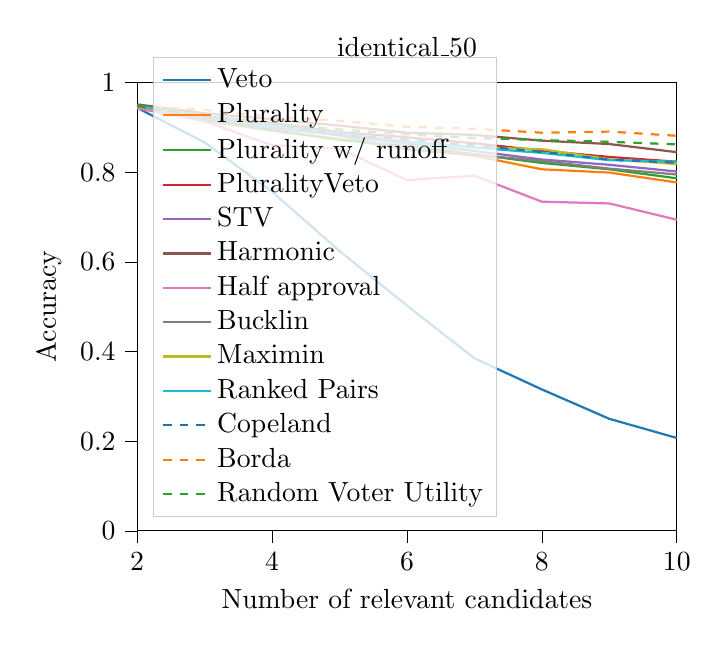
\begin{tikzpicture}

\definecolor{color0}{rgb}{0.12156862745098,0.466666666666667,0.705882352941177}
\definecolor{color1}{rgb}{1,0.498039215686275,0.0549019607843137}
\definecolor{color2}{rgb}{0.172549019607843,0.627450980392157,0.172549019607843}
\definecolor{color3}{rgb}{0.83921568627451,0.152941176470588,0.156862745098039}
\definecolor{color4}{rgb}{0.580392156862745,0.403921568627451,0.741176470588235}
\definecolor{color5}{rgb}{0.549019607843137,0.337254901960784,0.294117647058824}
\definecolor{color6}{rgb}{0.890196078431372,0.466666666666667,0.76078431372549}
\definecolor{color7}{rgb}{0.737254901960784,0.741176470588235,0.133333333333333}
\definecolor{color8}{rgb}{0.0901960784313725,0.745098039215686,0.811764705882353}

\begin{axis}[
legend cell align={left},
legend style={
  fill opacity=0.8,
  draw opacity=1,
  text opacity=1,
  at={(0.03,0.03)},
  anchor=south west,
  draw=white!80!black
},
tick align=outside,
tick pos=left,
title={identical\_50},
x grid style={white!69.0196078431373!black},
xlabel={Number of relevant candidates},
xmin=2, xmax=10,
xtick style={color=black},
y grid style={white!69.0196078431373!black},
ylabel={Accuracy},
ymin=0, ymax=1,
ytick style={color=black}
]
\addplot [thick, color0]
table {%
2 0.9434
3 0.8664
4 0.7563
5 0.6242
6 0.5024
7 0.3848
8 0.3154
9 0.2498
10 0.2071
};
\addlegendentry{Veto}
\addplot [thick, color1]
table {%
2 0.9497
3 0.9144
4 0.8922
5 0.8744
6 0.8514
7 0.8365
8 0.8064
9 0.7991
10 0.7771
};
\addlegendentry{Plurality}
\addplot [thick, color2]
table {%
2 0.9497
3 0.9185
4 0.8935
5 0.8719
6 0.8583
7 0.8399
8 0.8206
9 0.8064
10 0.7863
};
\addlegendentry{Plurality w/ runoff}
\addplot [thick, color3]
table {%
2 0.9476
3 0.9249
4 0.9096
5 0.8893
6 0.8777
7 0.8644
8 0.8479
9 0.8339
10 0.8233
};
\addlegendentry{PluralityVeto}
\addplot [thick, color4]
table {%
2 0.9469
3 0.921
4 0.8981
5 0.8825
6 0.8639
7 0.8473
8 0.8282
9 0.8164
10 0.8015
};
\addlegendentry{STV}
\addplot [thick, color5]
table {%
2 0.9512
3 0.9313
4 0.9181
5 0.9038
6 0.8881
7 0.8831
8 0.8702
9 0.8627
10 0.8446
};
\addlegendentry{Harmonic}
\addplot [thick, color6]
table {%
2 0.9423
3 0.9139
4 0.8598
5 0.8527
6 0.7823
7 0.7921
8 0.7341
9 0.7302
10 0.6939
};
\addlegendentry{Half approval}
\addplot [thick, white!49.8039215686275!black]
table {%
2 0.9468
3 0.9244
4 0.9033
5 0.8822
6 0.8505
7 0.8391
8 0.8248
9 0.8079
10 0.7948
};
\addlegendentry{Bucklin}
\addplot [thick, color7]
table {%
2 0.9459
3 0.9222
4 0.9044
5 0.8867
6 0.8682
7 0.8555
8 0.8511
9 0.8288
10 0.818
};
\addlegendentry{Maximin}
\addplot [thick, color8]
table {%
2 0.9487
3 0.9229
4 0.9032
5 0.8864
6 0.8672
7 0.8547
8 0.843
9 0.8267
10 0.8235
};
\addlegendentry{Ranked Pairs}
\addplot [thick, color0, dashed]
table {%
2 0.9469
3 0.9235
4 0.9088
5 0.8836
6 0.8726
7 0.8593
8 0.8452
9 0.8281
10 0.821
};
\addlegendentry{Copeland}
\addplot [thick, color1, dashed]
table {%
2 0.9464
3 0.939
4 0.9231
5 0.9145
6 0.9012
7 0.8967
8 0.888
9 0.8905
10 0.8811
};
\addlegendentry{Borda}
\addplot [thick, color2, dashed]
table {%
2 0.9479
3 0.9245
4 0.9086
5 0.8954
6 0.8843
7 0.8764
8 0.8715
9 0.8677
10 0.8619
};
\addlegendentry{Random Voter Utility}
\end{axis}

\end{tikzpicture}
